\documentclass[12pt]{article}

\usepackage[utf8]{inputenc}
\usepackage[T1]{fontenc}
\usepackage[polish,provide=*]{babel}
\usepackage{lmodern}
\usepackage{amsmath}
\usepackage{latexsym,amsfonts,amssymb,amsthm,amsmath}
\usepackage{enumitem}
\usepackage{hyperref}
\usepackage{float}
\usepackage{graphicx}
\usepackage{subcaption}
\usepackage{booktabs}
\graphicspath{{./images/}}

\setlength{\parindent}{0in}
\setlength{\oddsidemargin}{0in}
\setlength{\textwidth}{6.5in}
\setlength{\textheight}{8.8in}
\setlength{\topmargin}{0in}
\setlength{\headheight}{18pt}

\title{Przemiany Gazowe}
\author{Kacper Kłos}

\begin{document}

\maketitle

Abstract

\newpage
\section{Analiza Wyników}
\subsection{Czujniki i stałe}
W obu pomiarach będziemy korzystać z czujników ciśnienia PASCO PS-3203 o dokładności 2 kPa oraz czujnika temperatury PASCO PS-3222 z rozdzielczością 0{,}01 \(C^\circ\). Podczas wyznaczania wartości będziemy wykorzystywać stałą gazową\cite{gas_const} \(R = 8{,}314 \, mol^{-1} K^{-1}\).
\subsection{Przemiana Izohoryczna}
Pomiary zaczynamy od przemiany izohorycznej, gdzie w miedzianej sferze o promieniu 2 cali szczelnie zamknięta jest stała liczba moli powietrza. Wewnątrz sfery zawarte są wspomniane czujniki.



Przy pomocy otrzymanych danych jesteśmy w stanie oszacować temperature oraz liczbę moli zera bezwzględnego, zakładając że gaz w badanym zakresie zachowuje się jak gaz doskonały opisywany równaniem:
\[
    PV = nR(T + T_0)
\]
Gdzie \(P\), \(V\), \(n\), \(R\), \(T\), \(T_0\) oznaczają kolejno mierzone ciśnienie, objętośc gazu, liczba moli, stała gazowa, mierzona temperatura oraz temperatura zera bezwzględnego. Możemy zauważyć że niepewność ciśnienia na poziomie 2kPa oznacza okolice 2\% wartości naszych pomiarów ciśnienia, gdy błąt pomiaru temperatury na poziomie 0{,}5 \(C^\circ\)zaczyna się od około 2\%, lecz szybko maleje aż do 0{,}2\%. Wskazuje to że pomiar temperatury jest znacznie dokładniejszy, dlatego parametry będziemy dopasowywać do równania:
\[
    P = aT + b
\]
Otrzymujemy w ten sposób wykresy:
\begin{figure}[H]
    \centering
    \begin{subfigure}{0.47\textwidth}
        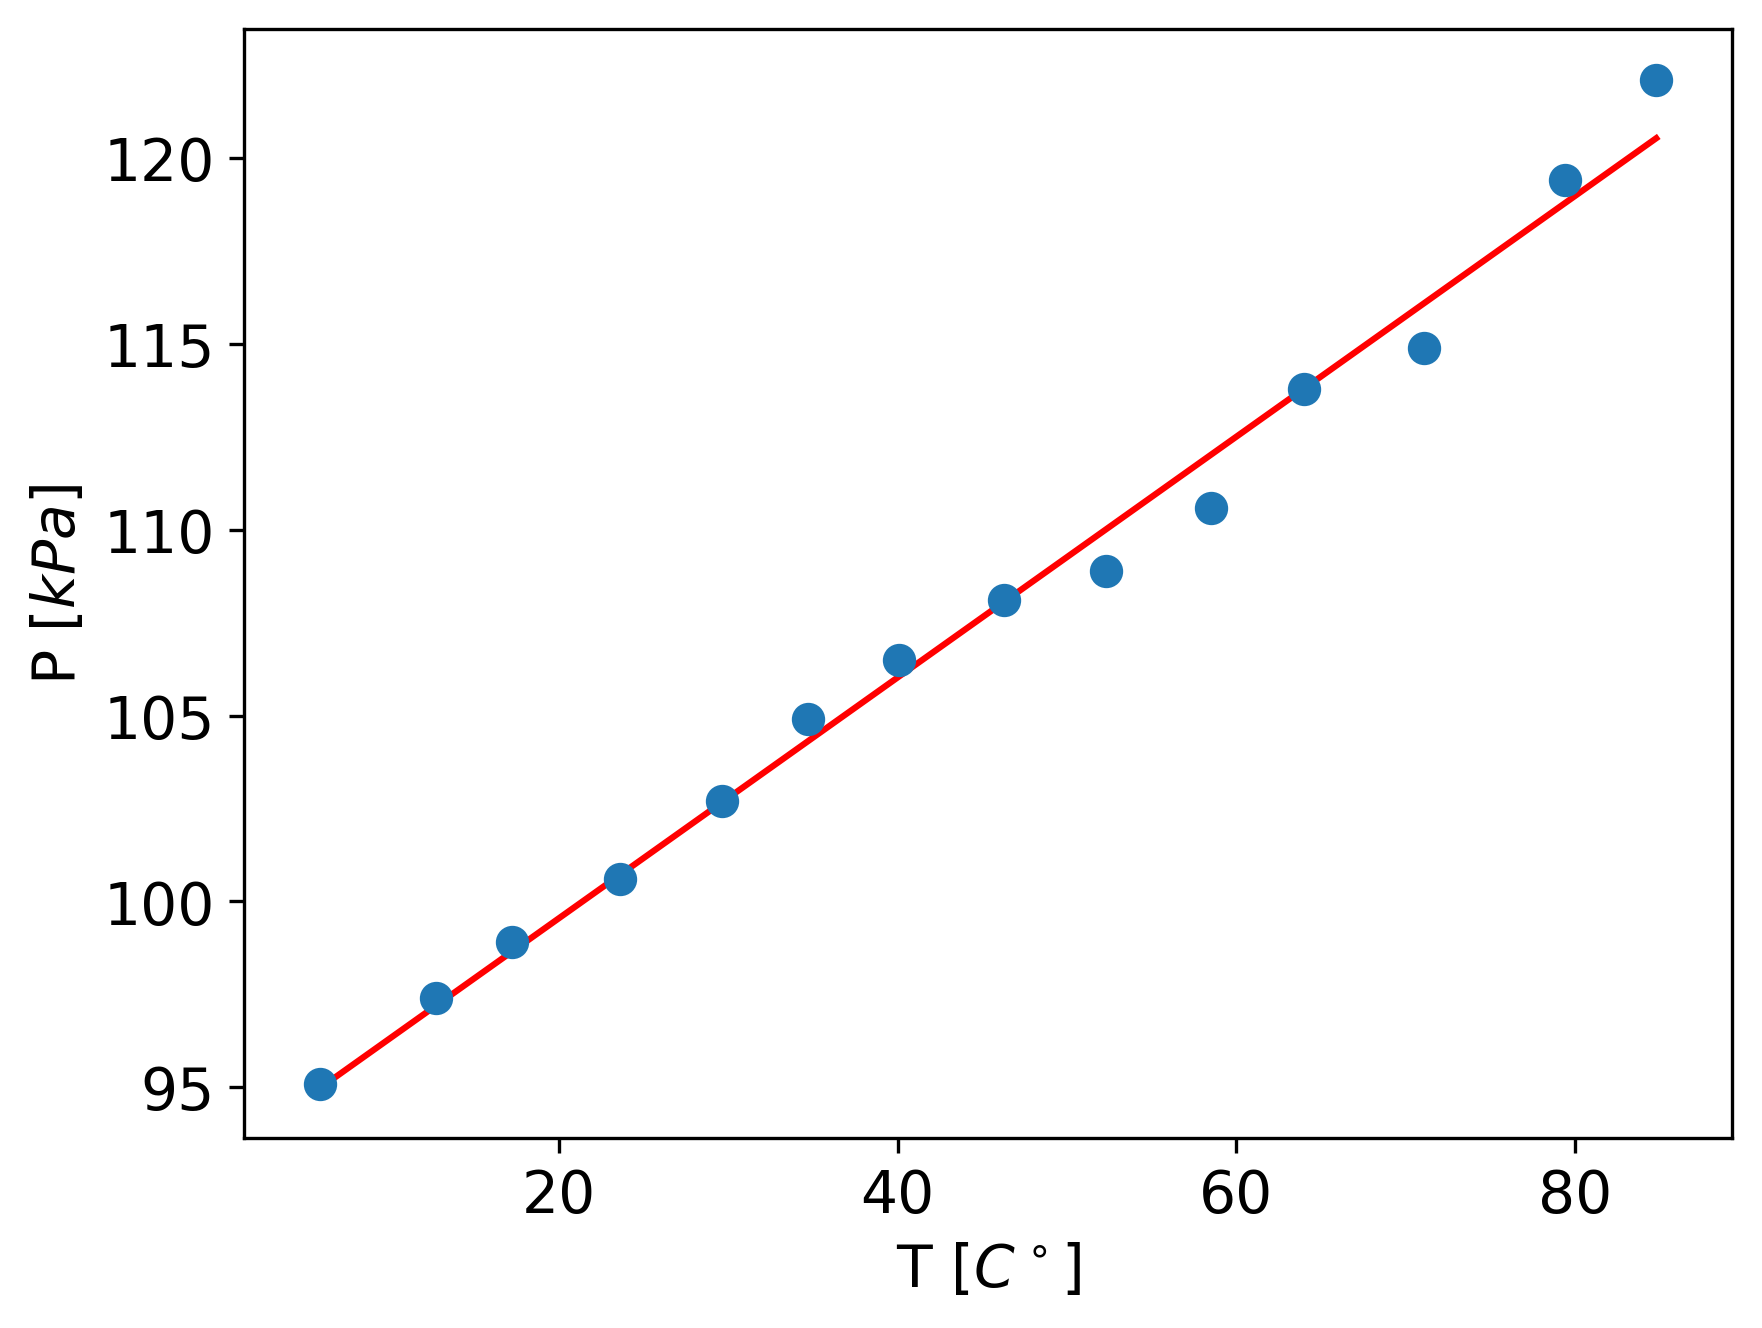
\includegraphics[width=\linewidth]{izohoric_0}
        \caption{1 seria pomiarowa}
    \end{subfigure}\hfill
    \begin{subfigure}{0.47\textwidth}
        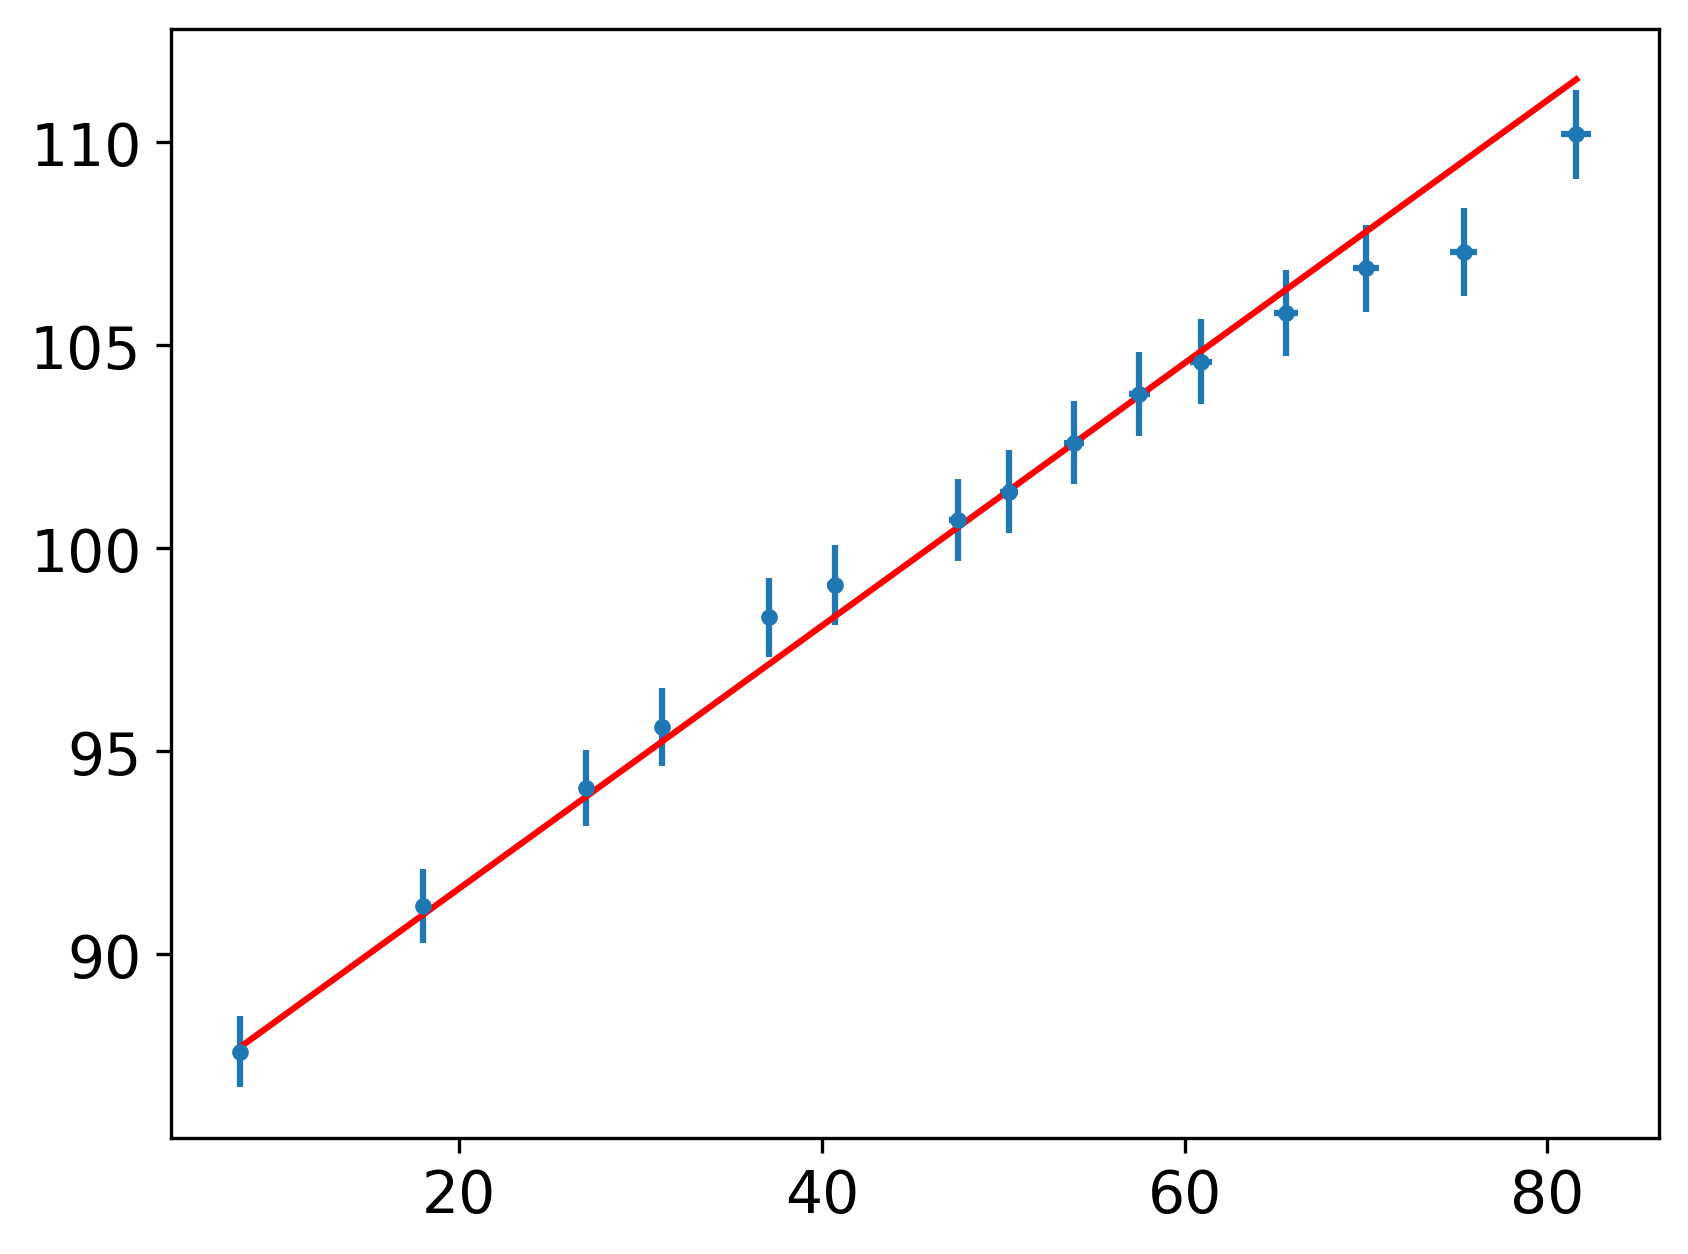
\includegraphics[width=\linewidth]{izohoric_1}
        \caption{2 seria pomiarowa}
    \end{subfigure}
    \caption{Zależność ciśnienia \(P\) od temperatury \(T\) w miedzianej kuli o stałej objętości \(V\)}
    \label{fig:izohoric}
\end{figure}
Gdzie parametry wynoszą
\[
    a_1 = , \quad b_1 = , \quad a_2 = , \quad b_2 =
\]
Z tych parametrów możemy otrzymać temperature zera bezwzględnego i liczbę moli
\[
    T_0 = \frac{b}{a}, \quad n = \frac{aV}{R}
\]
Co przy użyciu standardowego wzoru na objętość sfery przy promieniu 2 cali (1 cal = 2{,}54 cm) i wspomnianej już wartości stałej \(R\) skutkuje:
\[
    {T_0}_1 = ,\quad n_1 = ,\quad {T_0}_2 = ,\quad n_2 =
\]

\subsection{Przemiana Izotermiczna}
W tej części mierzyliśmy ciśnienie, temperature i objętość powietrzaw w strzykawce za podłączonymi wspomnianymi wyżej czujnikami ciśnienia oraz temperatury. Do końca strzykawki podłączyliśmy przewody które podpieliśmy do czujników.



Przy pomocy tych danych postaramy się oszacować w jakim zakresie powietrze zachowuje się jak gaz doskonały wyznaczając zależność:
\[
    \frac{P(V + V_0)}{T + T_0} = nR = \text{const}
\]
Gdzie symbole mają to samo znaczenie co w poprzedniej sekcji oraz \(V_0\) oznacza objętość powietrza zawartą w przewodach z gazem. W pomiarach dążyliśmy do tego aby temperatura pozosawała stale w okolicach \(T = (23{,}0 \pm 0{,}1)C^\circ\). Przekształcając to równanie na zależne od ciśnienia możemy zbadać zakres poprawności założenia że powietrze jest gazem doskonałym oraz wyznaczyć liczbę moli. Jako temperature zera bezwzględnego\cite{zero} przyjmujemy \(T_0 = 273{,}15\).
\[
    \frac{PV}{T + T_0} = aP + b
\]
Wyliczając te zależności otrzymujemy wykresy \ref{fig:izotermic} i ich dopasowania liniowe dla zakresów w którch zauważalna była taka zależność:
\begin{figure}[H]
    \centering
    \begin{subfigure}{0.47\textwidth}
        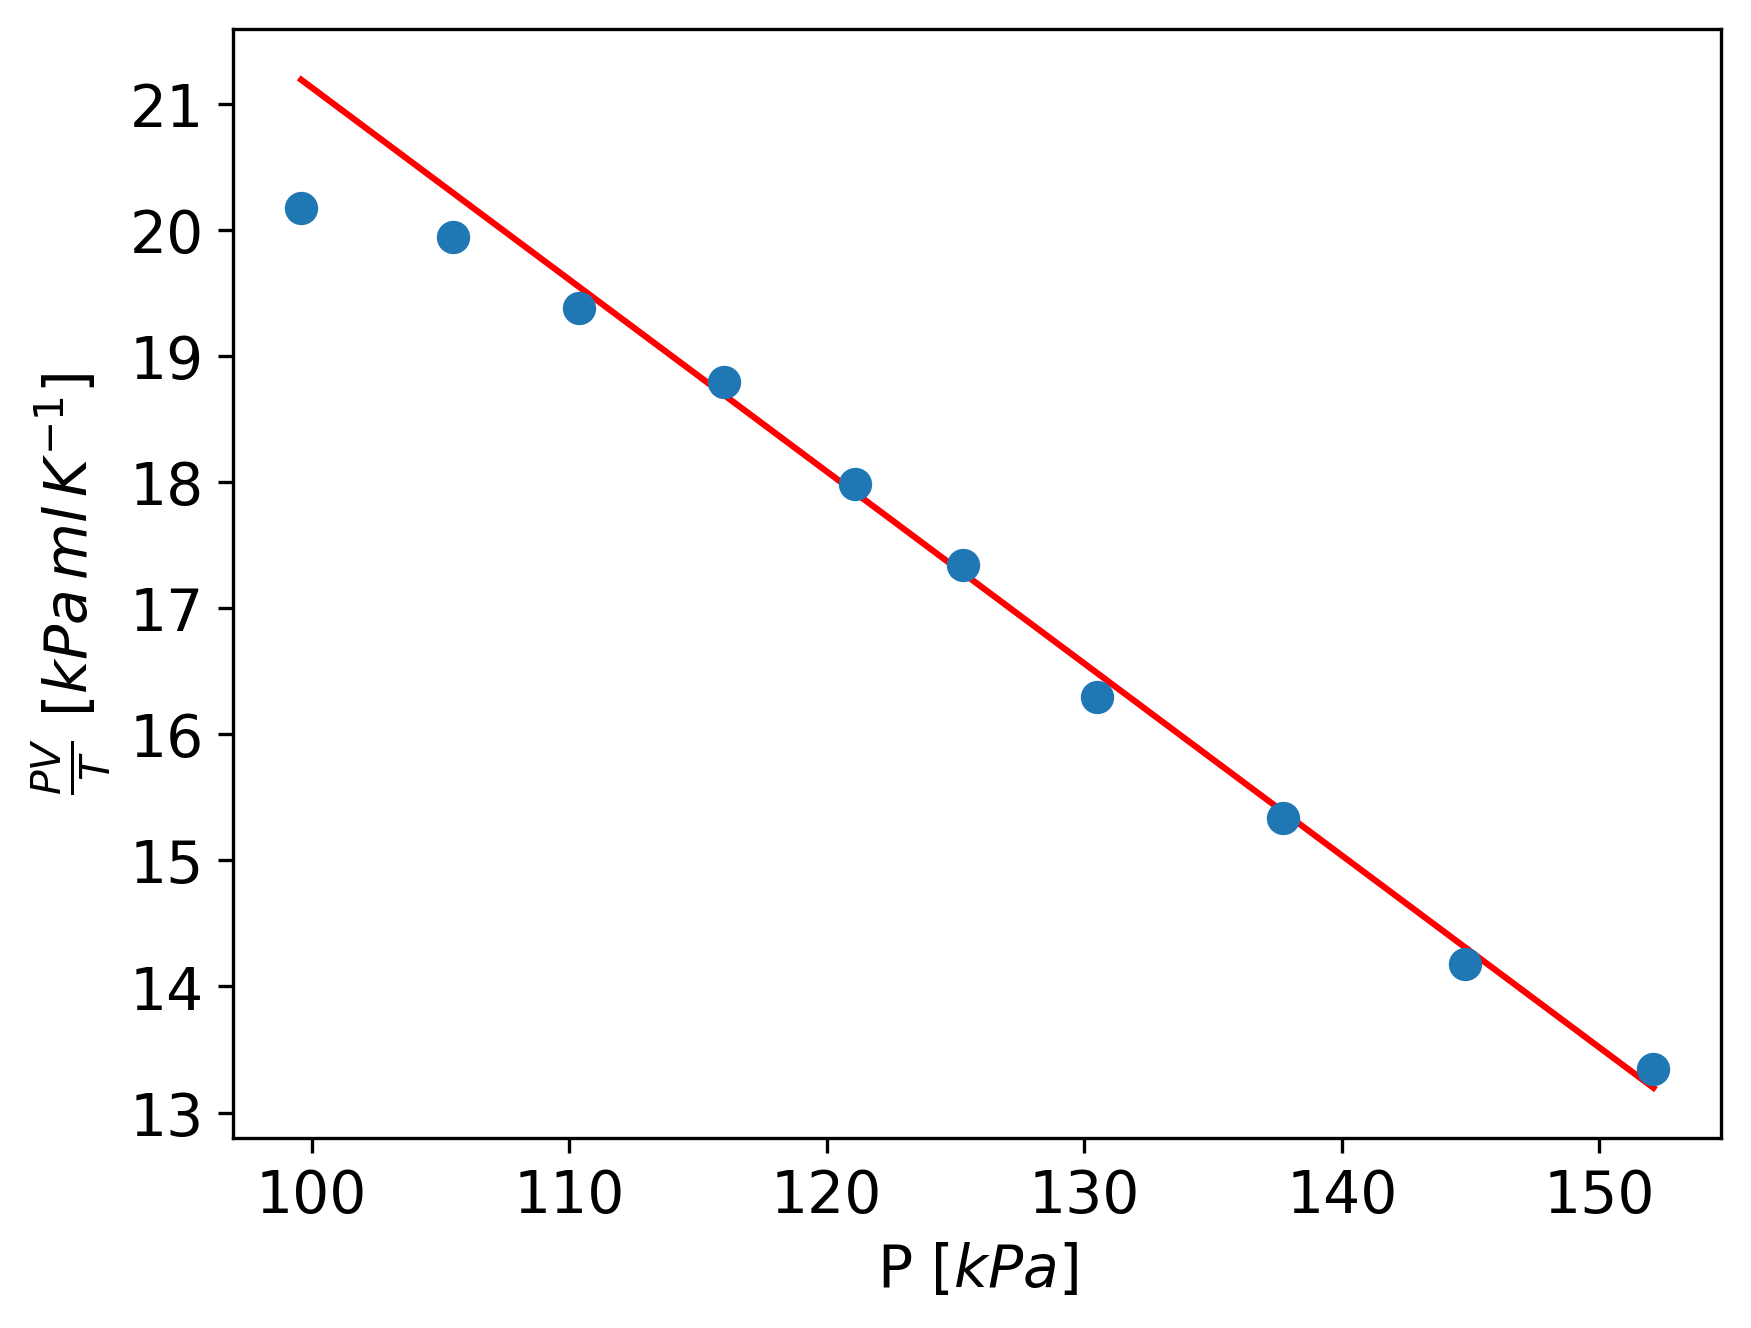
\includegraphics[width=\linewidth]{izotermic_0}
        \caption{1 seria pomiarowa}
    \end{subfigure}\hfill
    \begin{subfigure}{0.47\textwidth}
        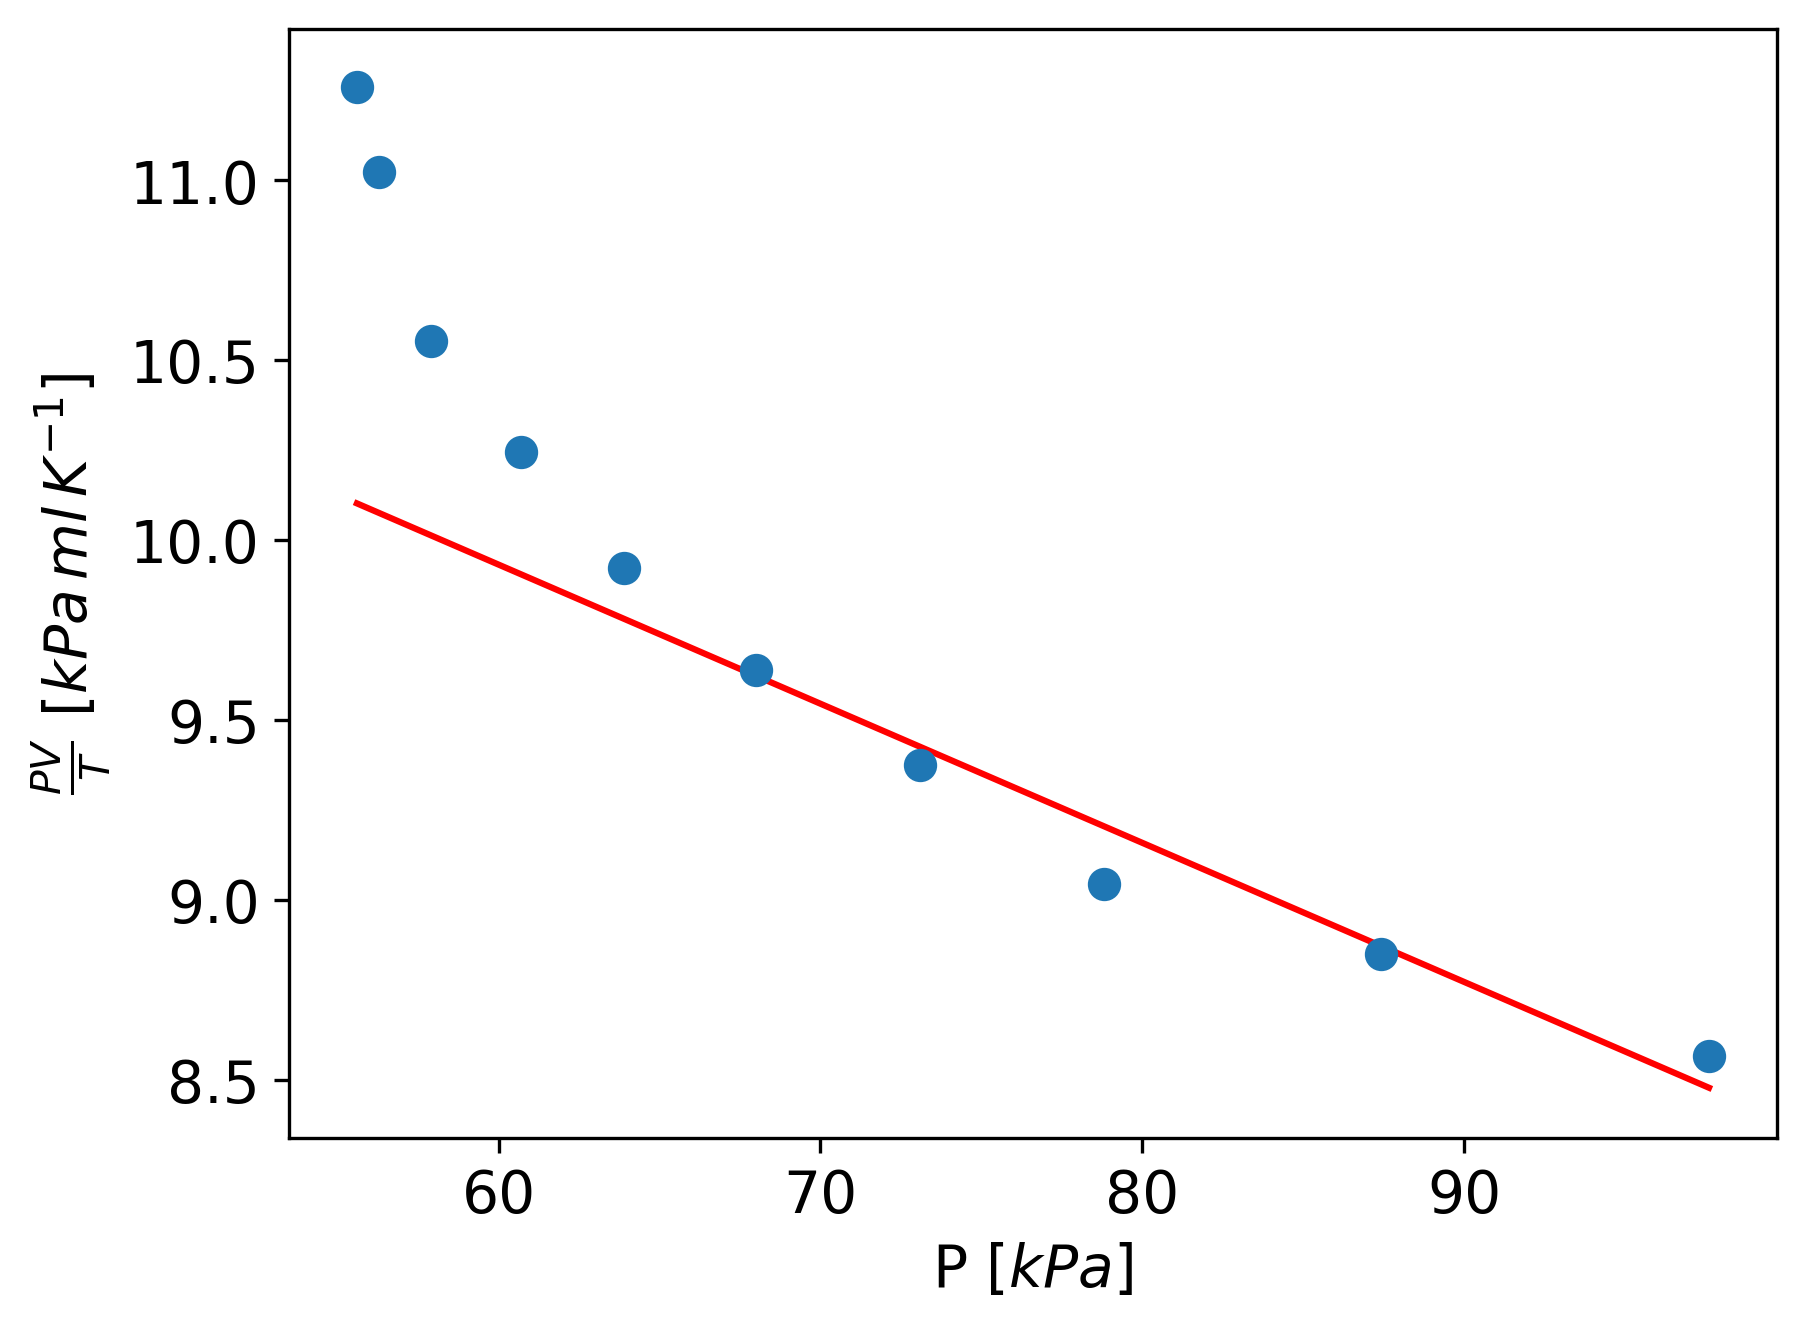
\includegraphics[width=\linewidth]{izotermic_1}
        \caption{2 seria pomiarowa}
    \end{subfigure}
    \caption{Wykres zależności \(\frac{PV}{T + T_0}\) od ciśnienia \(P\) przy stałej temperaturze \(T = (23{,}0 \pm 0{,}1)C^\circ\) dla dwóch różnych ilości molii zawartych w strzykawce.}
    \label{fig:izotermic}
\end{figure}
Gdzie w zakresach liniowych otrzymujemy parametry:
\[
    a_1 = , \quad b_1 = , \quad a_2 = , \quad b_2 =
\]
Za ich pomocą i wspomnianej wartości \(R\) możemy wyznaczyć liczbę moli:
\[
    n = \frac{b}{R}
\]
\[
    n_1 = ,\quad n_2 = 
\]

\section{Podsumowanie}

\begin{thebibliography}{1}

	\bibitem{skrypt}
	\emph{Interferencyjny Pomiar Krzywizny Soczewki (Pierścienie Newtona)}, Uniwersytet Warszawski.
    \bibitem{gas_const}
    \url{https://physics.nist.gov/cgi-bin/cuu/Value?r}
    \bibitem{zero}
    \url{https://www.bipm.org/documents/20126/41483022/SI-Brochure-9-EN.pdf/2d2b50bf-f2b4-9661-f402-5f9d66e4b507}

\end{thebibliography}


\newpage

\end{document}
